\chapter{Herramientas}
\label{chap:herramientas} 
En este capítulo se explica con un mayor grado de detalle qué herramientas han sido necesarias para el desarrollo del trabajo. Principalmente, se han utilizado los lenguajes de programación \textit{JavaScript, HTML, JSON, Python y Scratch}. Por otro lado, se han utilizado aplicaciones como \textit{Blender} para el modelado de objetos 3D y el simulador \textit{WebSim} para la recreación de los mundos tridimensionales.
   
\section{Lenguaje \textit{JavaScript}}
\textit{JavaScript} es un lenguaje de programación interpretado de alto nivel que se encuentra bajo el estándar \textit{ECMAScript}\footnote{Especificación de lenguaje de programación en el que se definen tipos dinámicos y soporte de programación oreintada a objetos}. Este lenguaje es comúnmente conocido por su uso en los scripts de las páginas web. No obstante, dada su orientación a objetos y a ser un lenguaje de programación basada en prototipos y de un solo hilo, es usado en otros muchos entornos externos de la página web: \textit{Node.js, Apache CouchDB o Adobe Acrobat}\footnote{https://developer.mozilla.org/es/docs/Web/JavaScript}. \newline

La sintaxis es similar a la utilizada en \textit{Java} y \textit{C++}. De esta manera, se facilita el aprendizaje del lenguaje ya que está basado en conceptos ya conocidos por el programador. Las estructuras del lenguaje, tales como sentencias condicionales (if y switch) y bucles (while y for), funcionan de una manera similar a como lo hacen en otros lenguajes de programación\footnote{\textit{https://developer.mozilla.org/es/docs/Web/JavaScript}}. \newline

Las siguientes características son las principales:
\begin{itemize}
    \item Lenguaje escructurado similar a la estructura utilizada en \textit{Java} y \textit{C++}.
    \item \textit{ECMAScript 2015} añadió la palabra clave \textit{let}, que permite que el alcance de la variable se corresponda con el bloque en el que esta se haya definido (\textit{block scoping}).
    \item Tipado débil, es decir, el tipo de datos se asocia al valor de la variable en un preciso momento.
    \item El lenguaje está formado por objetos.
    \item Lenguaje interpretado, es decir, se compila justo-a-tiempo. No es necesario disponer de un compilador adicional, cada navegador incluye un intérprete que se encarga de ejecutar el código.
\end{itemize}

Este TFG está enteramente programado en \textit{JavaScript}, ya que se trata de una aplicación web que corre en el lado del cliente. 

\section{Lenguaje \textit{HTML}}
\textit{HTML} es un lenguaje de marcado que define la estructura de una página web. \textit{HTML} ofrece una serie de elementos que permiten etiquetar diferentes partes de una misma página web en una misma clase para otorgarles una misma apariencia. Además, \textit{HTML} permite cambiar el estilo de las palabras (por ejemplo, a cursiva, a negrita, agrandar o reducir el tamaño de letra, etc)\footnote{https://developer.mozilla.org/es/docs/Learn/Getting$_$started$_$with$_$the$_$web/HTML$_$basics}. \newline

Las partes principales del elemento \textit{HTML} son las siguientes:
\begin{itemize}
    \item \textbf{Etiqueta de apertura:} se trata del nombre del elemento y se incluye entre paréntesis angulares $(< >)$. Indica el inicio del elemento.
    \item \textbf{Etiqueta de cierre:} similiar a la etiqueta de apertura salvo que incluye, además, una barra de cierre (/) precediendo al nombre de la etiqueta. Indica el fin del elemento.
    \item \textbf{Contenido: }todo aquello que se incluye entre la etiqueta de apertura y la de cierre.
    \item \textbf{Elemento: }es el conjunto formado por las etiquetas de apertura y cierre y el contenido del elemento.
\end{itemize}

Las etiquetas básicas de \textit{HTML} son la siguientes:
\begin{itemize}
    \item $<html>.$: comienzo del documento HTML.
    \item $<head>.$: cabecera de la página.
    \item $<body>.$:  cuerpo de la página.
    \item $<h1>, <h2>, etc.$: son los títulos o encabezados.
    \item $<a>.$: define los enlaces.
    \item $<table>.$: es una tabla.
    \item $<p>.$: define un párrafo.
    \item $<img>.$: imágenes.
    \item $<ul>.$: define una lista.
\end{itemize}

   


Además, cada elemento puede incluir uno o más atributos que permiten añadir mas información acerca de ese elemento. Por ejemplo, añadir información sobre el estilo del elemento. A continuación, se incluye un fragmento de código \textit{HTML} a modo de ejemplo. 
\begin{verbatim}
<!DOCTYPE html>
<html>
  <head>
    <meta charset="utf-8">
    <title>Mi código de prueba</title>
  </head>
  <body>
    <p class="editor-note">Esto es<strong>una prueba</strong></p>
  </body>
</html>
\end{verbatim}

\textit{Kibotics} emplea \textit{HTML} para crear las plantillas de las diferentes páginas que sirve la aplicación web.

\section{Lenguaje \textit{JSON}}
El acrónimo \textit{JSON} significa JavaScript Object Notation (Notación de Objetos de JavaScript). Se trata de un formato para el intercambio de datos. Es un lenguaje sencillo para la escritura y lectura humana y, al mismo tiempo, resulta fácil para las máquinas interpretarlo y procesarlo. \textit{JSON} está constituído por dos estructuras: una colección de pares nombre - valor y una lista ordenada de valores. Dado que estas convenciones son conocidas por otros lenguajes como  \textit{C, C++, C#, Java, JavaScript, Perl, Python}, se trata de un lenguaje ideal para el intercambio de datos\footnote{https://www.json.org/json-es.html}. \newline


En \textit{JSON}, estas estrucutras se presentan de la siguiente forma:
\begin{itemize}
    \item \textbf{Objeto: } conjunto desordenado de pares nombre - valor. Un objeto va encerrado entre llaves ({ }). La sintaxis es la siguiente: 
    \begin{verbatim}
        objeto {
            nombre1: valor1,
            nombre2: valor2,
            ...
        }
    \end{verbatim}
    \item \textbf{Array: } colección de valores. Van encerrados entre corchetes [ ]. Un valor puede ser una cadena de caracteres con comillas dobles, un número, true, false o null, un objeto o un array. Estas estructuras pueden anidarse.

\end{itemize}

La plataforma \textit{Kibotics} emplea \textit{JSON} para los ficheros de configuración de los diferentes escenarios utilizados en los ejercicios que ofrece la aplicación. Mediante un \textit{parser} se recopila la información necesaria del fichero de configuración \textit{JSON} para construir el mundo en \textit{A-Frame}.

\section{\textit{Blender}}
\textit{Blender}\footnote{https://www.blender.org/} es un programa informático multi plataforma, es decir, compatible para distintos sistemas operativos como Windows o Linux. Las funciones principales que se pueden realizar con \textit{Blender} son el modelado, iluminación, renderizado, animación y creación de gráficos tridimensionales. También se pueden realizar actividades relacionadas con la composición de vídeo. 

\begin{figure}[h!]
    \centering
    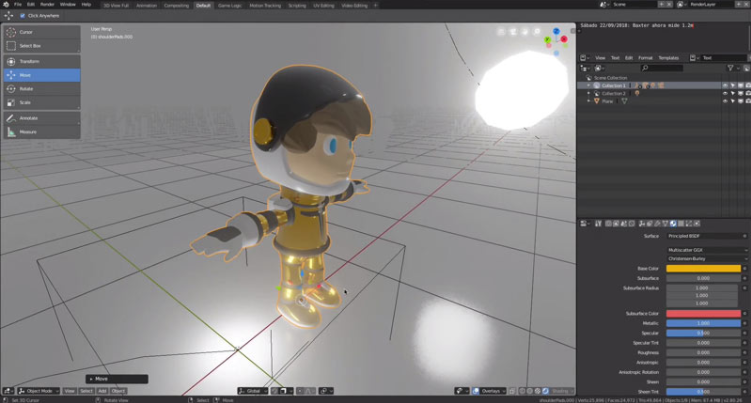
\includegraphics[scale=0.7]{blender.PNG} 
    \caption{Interfaz de trabajo con \textit{Blender}}
    \label{fig:blender}
\end{figure}

Durante el presente trabajo se ha utilizado esta herramienta para modificar la rotación y apariencia de los robots de los que dispone la plataforma \textit{Kibotics}. Además, \textit{Blender} permite exportar los modelos en formato glTF (GL Transmission Format). glTF es un formato de archivo basado en el estandar \textit{JSON}. Permite la compresión de escenas y modelos 3D para minimizar el tiempo de ejecución de los programas en los que posteriormente se utilicen.

\section{Entorno \textit{A-Frame}}
A-Frame es un marco web para crear escenas de realidad virtual en el navegador. Ha sido utilizado por empresas como \textit{Google, Disney, Samsung, Toyota} o \textit{CERN}, entre otras. Además, algunas de ellas, como \textit{Google, Microsoft, Oculus} y \textit{Samsung} han llegado a realizar contribuciones. Sus principales características son las siguientes\footnote{https://aframe.io/docs/1.0.0/introduction/#features}:

\begin{itemize}
    \item \textbf{Permite un uso sencillo de la realidad virtual:} para usar \textit{A-Frame} basta con colocar las etiquetas $<script>$ y $<a-scene>$. A-Frame se encarga del modelado 3D y la realidad virtual, no es necesaria la instalación de ningún paquete externo.
    \item \textbf{\textit{HTML} declarativo:} \textit{A-Frame} está basado en \textit{HTML}, por ello es fácil y accesible para cualquier programador, puesto que HTML es un lenguaje ampliamente conocido.
    \item \textbf{Arquitectura de componente de entidad:} \textit{A-Frame} sigue el patrón \textit{ECS} (entidad-componente-sistema). Se trata de un patrón de desarrollo de juegos basado en el principio de composición sobre herencia. De esta manera, se otorga una mayor flexibilidad en la definición de entidades ya que cada objeto de la escena se corresponde con una entidad y cada entidad, a su vez, está compuesta por uno o más componentes que contienen datos y estado de la entidad. Por tanto, una entidad puede verse modificada en tiempo de ejecución si alguno de los componentes que agrega modifica sus datos.
    \item \textbf{Multiplataforma: } \textit{A-Frame} es compatible con plataformas tan variadas como \textit{Vive, Rift, Windows Mixed Reality, Daydream, GearVR y Cardboard}.
    \item \textbf{Rendimiento:} las actualizaciones de \textit{A-Frame} se realizan en la memoria y con poco gasto energético. A-Frame se encuentra optimizado para \textit{WebVR}.
    \item  \textbf{Inspector visual:} \textit{A-Frame} cuenta con un inspector visual integrado. Este se despliega al presionar la combinación de teclas $<ctrl>$ + $<alt>$ + $i$. El inspector permite detectar el origen de problemas o desarrollar una mejor distribución de la escena con menos esfuerzo.
    \item \textbf{Componentes:} \textit{A-Frame} cuenta con una gran cantidad de componentes con los que trabajar. Esta amplia variedad va desde componentes geométricos básicos o materiales hasta componentes como la teletransportación, la realidad aumentada o componentes personalizados por el usuario.
\end{itemize}

\begin{figure}[h!]
    \centering
    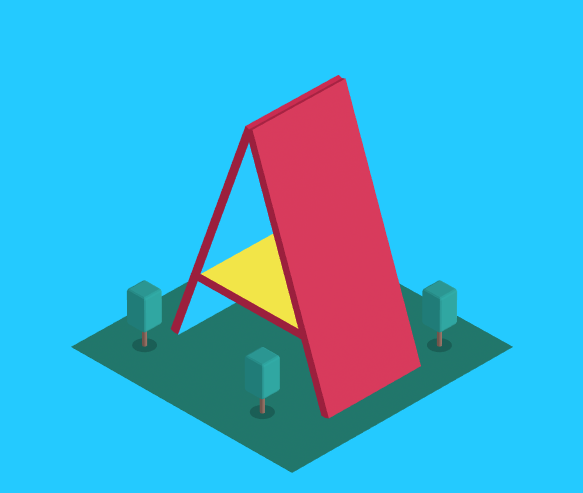
\includegraphics[scale=0.75]{a-frame.PNG} 
    \caption[Ejemplo de construción 3D con \textit{A-Frame}]{Ejemplo de construción 3D con \textit{A-Frame} \footnotemark}
    \label{fig:a-frame}
\end{figure}
\footnotetext{https://aframe.io/}

\subsection{Sistema de físicas de \textit{A-Frame}}
Las físicas de \textit{A-Frame} soportan dos motores de físicas: \textit{Ammo Driver y CANNON}. Actualmente, el motor que está en uso por defecto es el de \textit{CANNON}\footnote{https://github.com/donmccurdy/aframe-physics-system}. No obstante, ya ha sido añadido el soporte de \textit{Ammo.js} al sistema de físicas, y se preveé que \textit{CANNON} acabe quedando obsoleto con el paso del tiempo. \newline

Para la instalación del sistema de físicas de \textit{A-Frame} basta con incluir el siguiente script en el código \textit{HTML} de la aplicación: 

\begin{verbatim}
<script src="//cdn.rawgit.com/donmccurdy/aframe-physics-system/v4.0.1/  
dist/aframe-physics-system.min.js"></script>
\end{verbatim}

El sistema de físicas de \textit{A-Frame} cuenta con dos tipos de cuerpos: dinámicos y estáticos.

\begin{itemize}
    \item \textbf{Cuerpo dinámico:} aquellos objetos de la escena que presentan libertad de movimiento. Estos objetos se ven afectados por la gravedad, la fricción y las colisiones.
    \item \textbf{Cuerpo estático:} aquellos objetos de la escena que no necesitan modificar su posición en la misma. Son cuerpos fijos y sin animaciones. Otros cuerpos dinámicos podrán colisionar con un cuerpo estático, pero el cuerpo estático no verá modificada su posición tras la colisión.
\end{itemize}

El sistema de físicas ofrece la posibilidad de añadir una malla de colisión a un objeto de la escena. Existen mallas de colisión de diferentes formas, por lo que se debe seleccionar aquella que se ajuste mejor al objeto en cuestión. Se puede elegir entre el ajuste automático, una caja, un cilindro, una esfera, un cuerpo convexo o una primitiva ( plano, cilindro o esfera seleccionadas automáticamente en función de la primitiva \textit{A-Frame} correspondiente). \newline


Cada escena de  \textit{A-Frame}  admite una serie de parámetros a los que se les puede modificar el valor para ajustar el mundo a las características deseadas. Si no se especifica el valor que se desea de un parámetro, este tomará el valor por defecto. Algunos de los parámetros que admite una escena son \textit{debug}, que cuando está a \textit{true} muestra las mallas de colisión de los objetos de la escena o \textit{gravity, friction y restitution}, que se corresponden con la gravedad, fricción y coeficiente de restitución, respectivamente, del mundo simulado.
\begin{table}[h!]
\centering
\begin{tabular}{|c|c|}
\hline
\textbf{Atributo}    & \textbf{Valor por defecto} \\ \hline
debug       & true              \\ \hline
gravity     & -9.8              \\ \hline
friction    & 0.01              \\ \hline
restitution & 0.3               \\ \hline
\end{tabular}
\caption{Parámetros configurables del sistema de físicas de \textit{A-Frame}}
\label{fig:param-fisicas}
\end{table}

\section{Plataforma \textit{Kibotics}}
La batería de ejercicios que incluye el entorno \textit{Kibotics} se ejecuta usando el simulador robótico \textit{Websim}. Se trata de un simulador diseñado para el aprendizaje de conceptos básicos de programación de robots especialmente para niños. El simulador permite que los usuarios puedan programar fácilmente los movimientos de los robots, ya que simplemente tienen que acceder a la información que recogen sus sensores y enviar las órdenes precisas a los actuadores del robot. Estas órdenes se deberán programar, en\textit{ Python o Scratch}, dentro del editor que incorpora la interfaz de \textit{Websim}. \newline

El simulador está diseñado basándose en el uso del entorno \textit{A-Frame}. A su vez, \textit{A-Frame} se sirve del motor de físicas de \textit{CANNON} para materializar los movimientos de los cuerpos dinámicos en la escena.

\begin{figure}[h!]
    \centering
    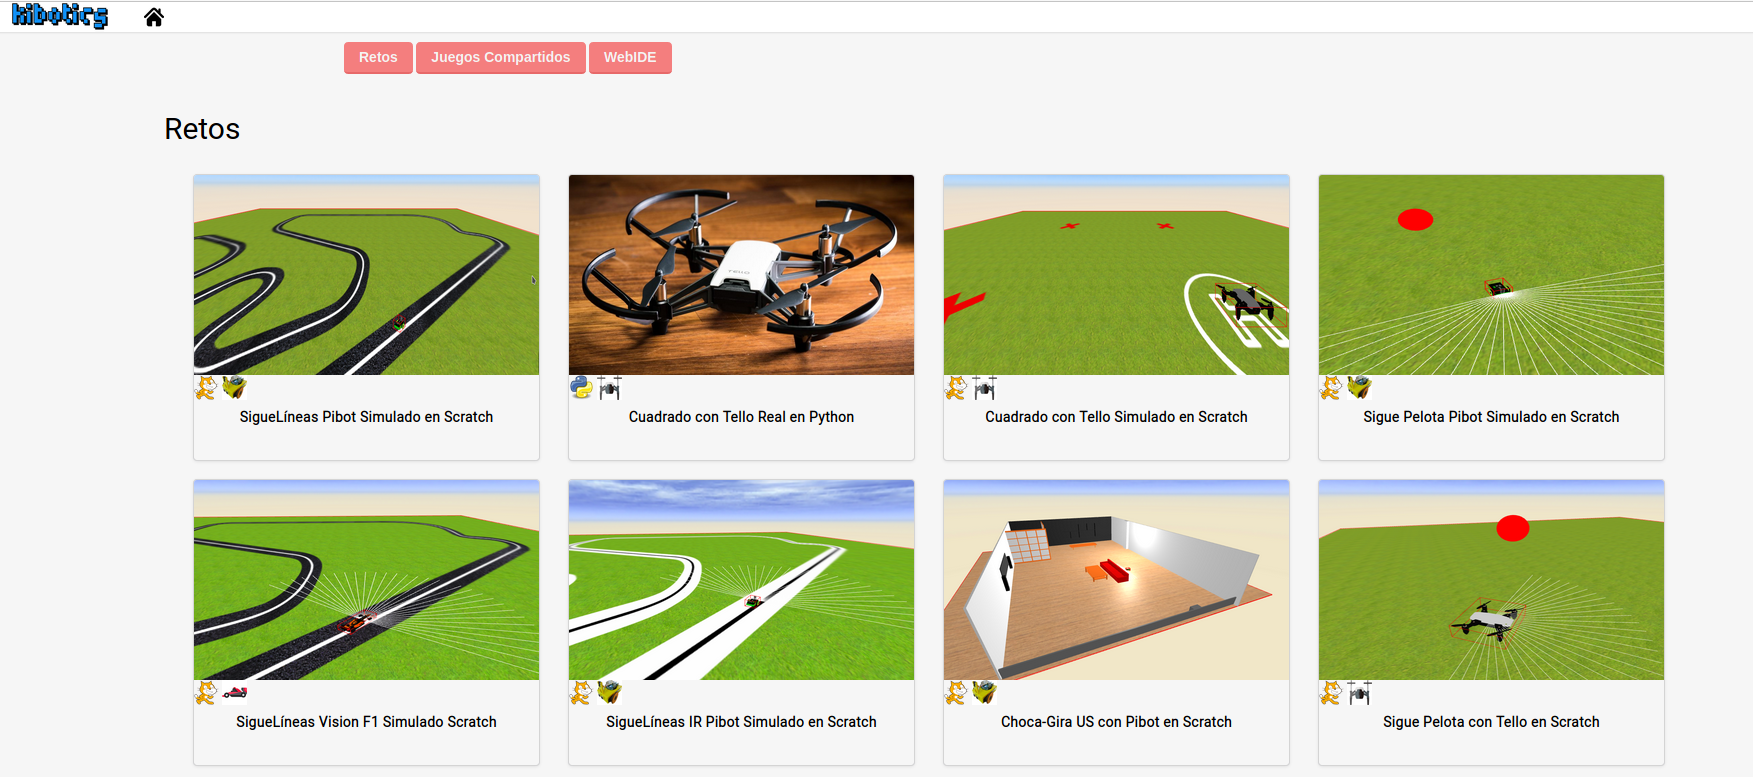
\includegraphics[scale=0.25]{kibotics.png} 
    \caption{Menú de ejercicios de \textit{Kibotics}}
    \label{fig:kibotics}
\end{figure}

\begin{figure}[h!]
    \centering
    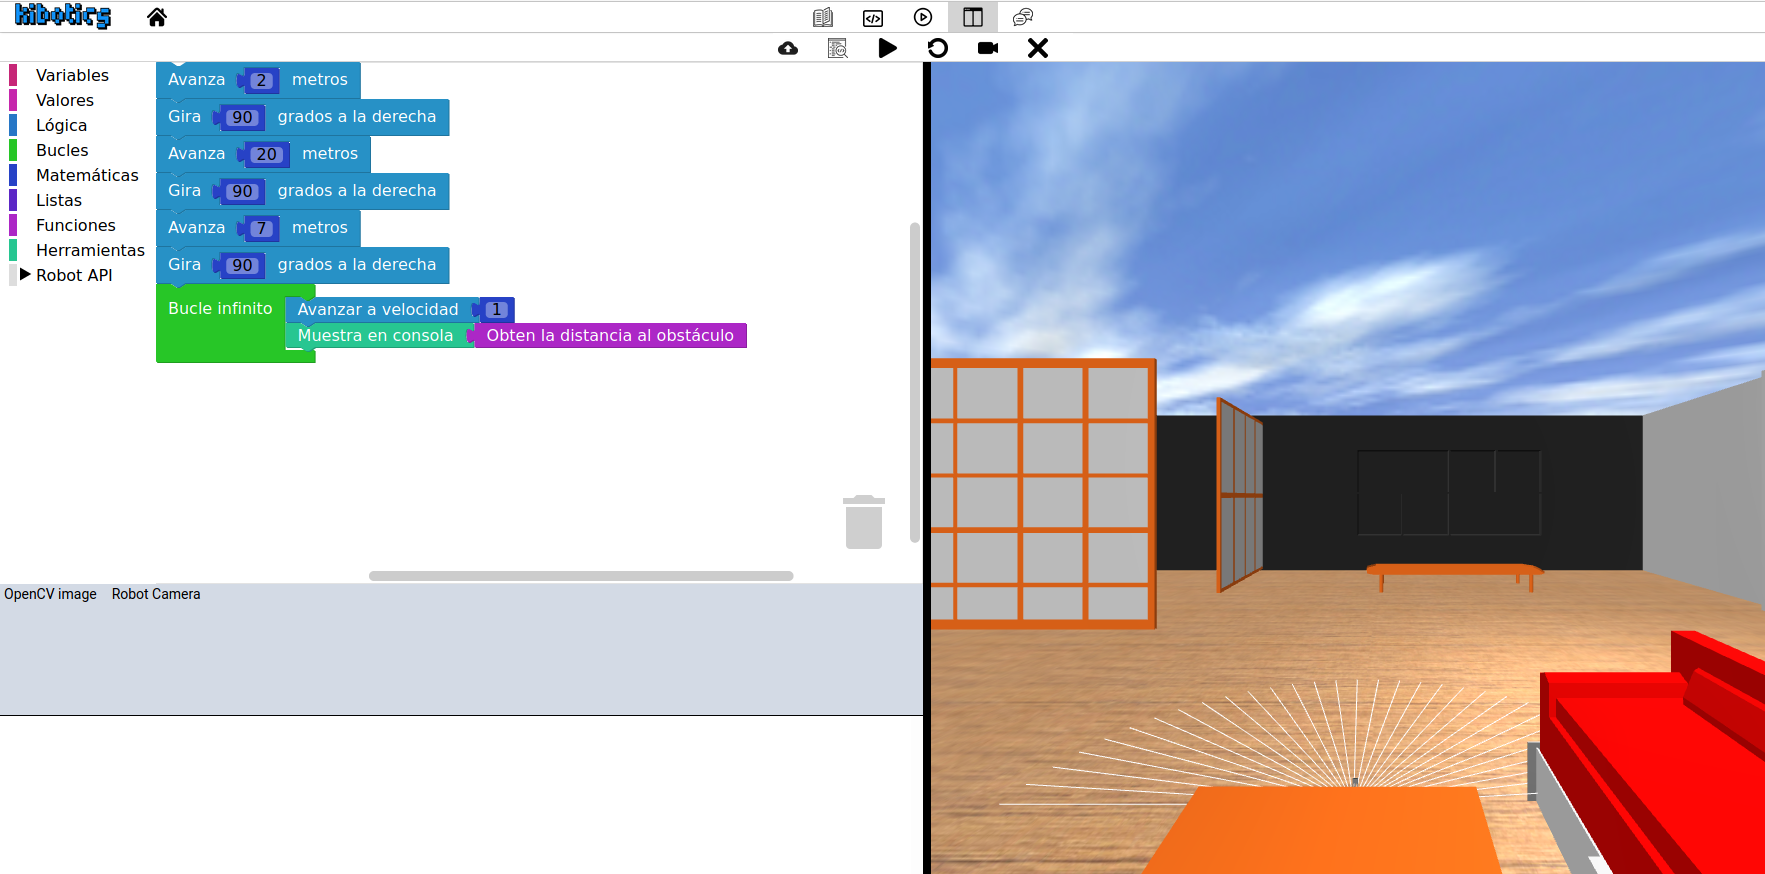
\includegraphics[scale=0.25]{scratch.png} 
    \caption{Editor \textit{Scratch} en \textit{WebSim}}
    \label{fig:scratch}
\end{figure}

\begin{figure}[h!]
    \centering
    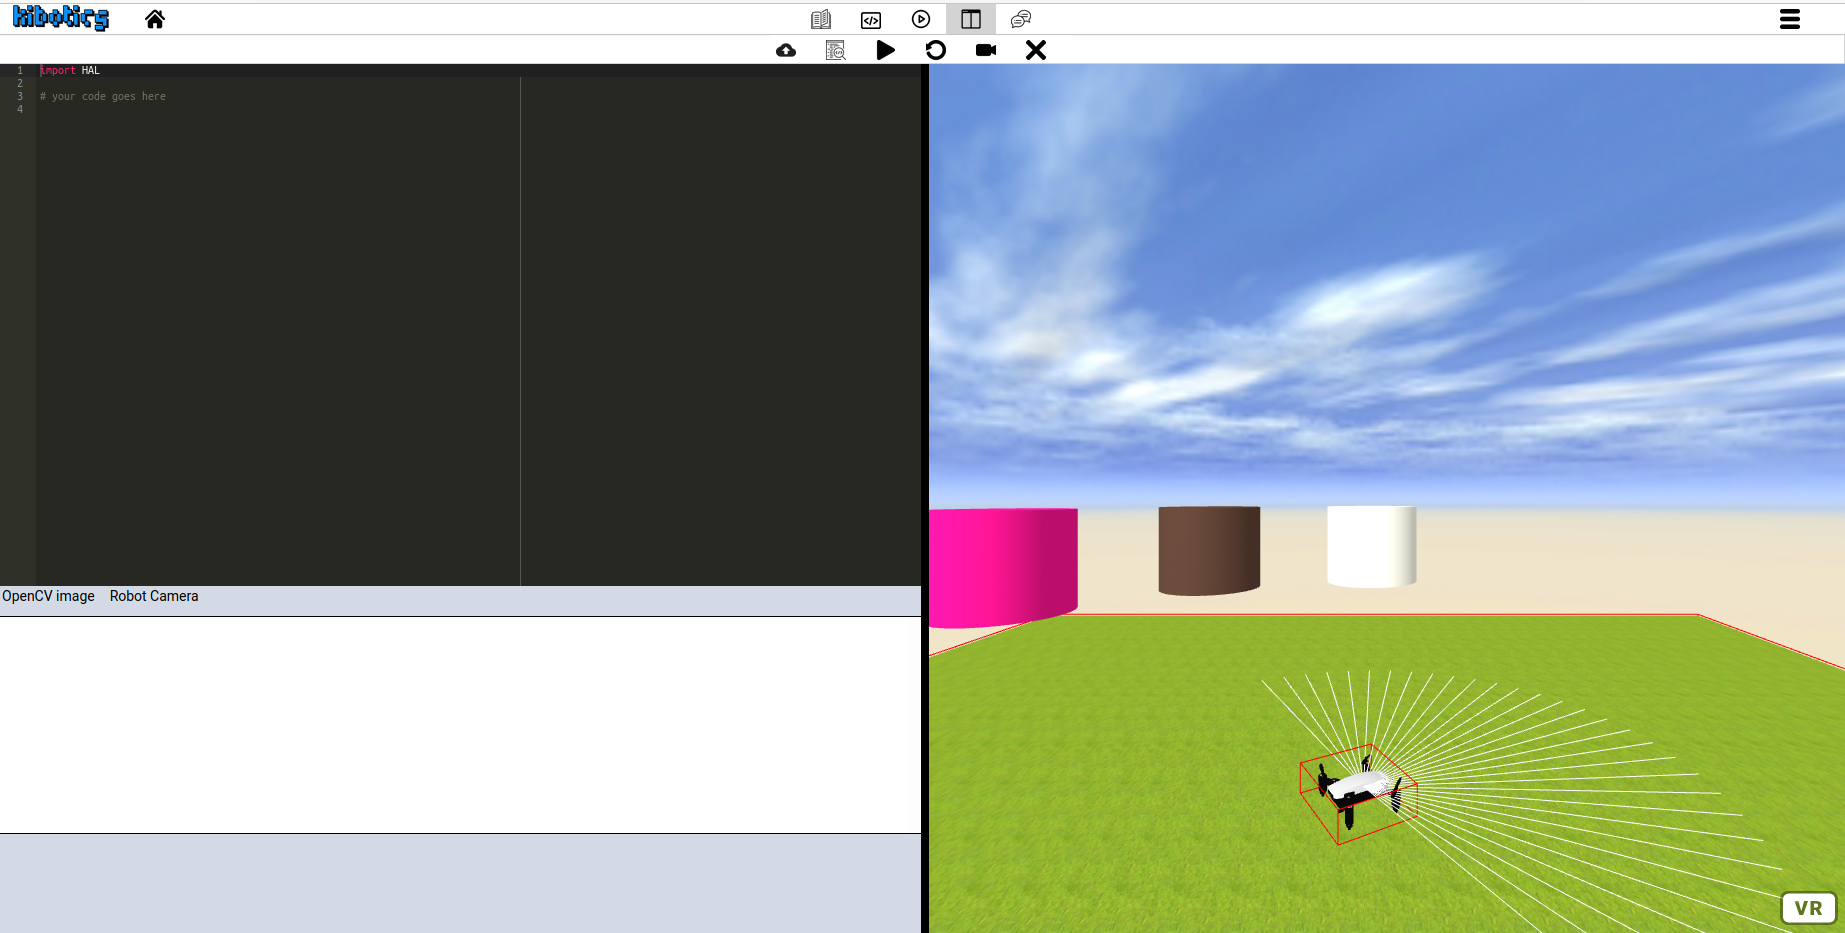
\includegraphics[scale=0.25]{python.png} 
    \caption{Editor \textit{Python} en \textit{WebSim}}
    \label{fig:python}
\end{figure}